\IEEEraisesectionheading{\section{Introduction}\label{intro:sec}}
\IEEEPARstart{L}{anguage-model} agents act through tools with irreversible effects (email,
payments, file edits) while reading untrusted content, so an attacker who
controls that content can steer the next tool call
\citep{greshake2023injection}. A common defense is a runtime guardrail: a
judge, often itself a language model, scores each proposed call, and a gate
blocks, rewrites, or escalates it before it executes
\citep{inan2023llamaguard,chennabasappa2025llamafirewall,agentspec2026,probguard2025,veriguard2025,agentc2025,wu2026provably}.
This gate is the security boundary between an injectable agent and
irreversible effects (Figure~\ref{fig:overview}). In the dependability
taxonomy of \citet{avizienis2004basic}, the gate is an error-detection and containment
mechanism in front of irreversible service: each miss lets a security or safety failure
through, and each false block is an omission failure that costs availability. Whether the
gate can justifiably be trusted therefore depends both on its error rates and on the fault
assumptions under which they are claimed.


Benchmark violation and false-positive rates do not say which policies a
gate can enforce at all, what a calibrated ``certificate'' guarantees, or
when that guarantee stops holding. For programs, the first question has a
classical answer: execution
monitors enforce only safety properties \citep{schneider2000enforceable}, and edit
automata enforce more by suppressing and reinserting actions
\citep{ligatti2005edit}. Agent gates depart from that setting in four ways: a fallible judge
decides the policy predicate (``does this body contain PII?''); effects are
irreversible, so the gate cannot buffer and retract as an edit automaton does, which
returns it to the execution-monitor (safety) regime of \citet{schneider2000enforceable};
actions carry unbounded data, which security automata already admit over countable
alphabets but which a deployed gate must represent finitely; and the attacker controls
part of what the judge sees. The safety half of our first result is therefore classical;
its contribution is the effect-trace, oracle-relative, register-automaton form:
characterizing the class a monitor with restricted state enforces is classical over finite
alphabets \citep{fong2004shallow,talhi2008memory}, and we carry it to keyed-counter register
automata over infinite data alphabets, relative to oracle bits. Each result states where it applies. ``Certified'' means
streamwise enforcement relative to fixed oracle predicates, or a marginal risk
bound under explicit stochastic assumptions, never universal semantic safety.

\begin{example}[Running example: an email/payments assistant]\label{ex:running}
An assistant acts for a user through tools such as
$\mathsf{send\_email}(\mathit{to},\mathit{body})$ and
$\mathsf{transfer}(\mathit{to},\mathit{amount})$, under three policies:
(P1)~never email a body containing PII to a recipient not on the approved list;
(P2)~never let cumulative transfer to any recipient exceed cap $c$ in a day bucket set by a trusted clock;
(P3)~after the user revokes access, send nothing further. P2 and P3 are
oracle-checkable data-carrying properties; P1 rests on the semantic predicate
``contains PII,'' which only a fallible judge evaluates.
\end{example}

\begin{figure}[t]
\centering
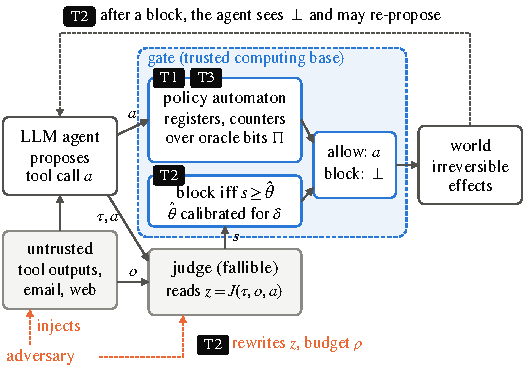
\includegraphics[width=\columnwidth]{overview}
\caption{A guarded tool-using agent. The agent, partly steered by untrusted input, proposes a
data-carrying tool call $a$. The gate (the trusted computing base) combines a policy automaton over
oracle bits $\Pi$ with a threshold test on a fallible judge's score $s$ of the judge-visible input $z$,
and either commits $a$ irreversibly or blocks it by committing the no-op $\bot$. T1: what the automaton
can enforce. T2: what a judge-based test can certify (frontier, calibration of $\hat\theta$, budget-$\rho$
rewrites of $z$, feedback). T3: whether a rule can ever fire, decided before deployment.}
\label{fig:overview}
\end{figure}

\paragraph{Three boundaries}
\emph{T1, expressiveness (\S\ref{sec:t1}).} Relative to fixed oracle predicates, a deterministic gate
enforces exactly the nonempty safety policies whose good prefixes its register automaton recognizes
(Theorem~\ref{thm:t1}), strictly fewer than edit automata (Proposition~\ref{prop:strict}): a gate that
cannot retract must refute violations on finite prefixes. P2 and P3 are inside this class; P1 needs a judge.
\emph{T2, statistics, adversaries, and feedback (\S\ref{sec:t2}).} With a judge, Neyman--Pearson gives the
exact miss/false-block frontier of the gate's information (Proposition~\ref{thm:frontier}) and conformal
risk control a finite-sample certificate (Theorem~\ref{thm:conformal}) that may be block-all; rewrites of
the judge's input within budget $\rho$ add a margin (Theorem~\ref{thm:adv}); once blocks change later
proposals, static scores and ungated logs cannot identify the closed-loop frontier
(Proposition~\ref{prop:feedback}), whereas exploratory blocking logs can, at a variance that may grow
exponentially in the horizon (Proposition~\ref{prop:explore}).
\emph{T3, decidability (\S\ref{sec:t3}).} Whether a rule can ever fire is undecidable with two
zero-testable counters (Proposition~\ref{thm:undec}), \PSPACE-complete for a keyed-counter fragment with data
registers, and \NP-complete for caps, quotas, and revocation without them, so one SMT query lints them (Theorem~\ref{thm:frag}). Table~\ref{tab:summary} gives each result's regime and what is
imported versus new.

% Summary of the three boundaries (journal version): what each result says, when it holds,
% what is imported versus new, and what it means for a deployment.
\begin{table*}[t]
\caption{The three boundaries at a glance. Each result holds only in its stated regime; the
evidence column points to the experiment that probes it.}
\label{tab:summary}
\centering\footnotesize
\setlength{\tabcolsep}{4pt}
\renewcommand{\arraystretch}{1.12}
\begin{tabularx}{\textwidth}{@{}>{\raggedright\arraybackslash}p{0.255\textwidth}>{\raggedright\arraybackslash}p{0.15\textwidth}>{\raggedright\arraybackslash}X>{\raggedright\arraybackslash}X>{\raggedright\arraybackslash}p{0.062\textwidth}@{}}
\toprule
Boundary and result & Regime & Imported ingredient $\rightarrow$ what is new & Consequence for deployments & Evidence\\
\midrule
\textbf{T1 expressiveness} (Thm.~\ref{thm:t1}, Prop.~\ref{prop:strict}): a deterministic gate
enforces exactly the nonempty safety policies with $\Good(P)\in\RA[\Th;\Pi]$, strictly fewer than
edit automata
& fixed oracle bits $\Pi$; irreversible commits; every proposal stream
& security, truncation, and bounded-memory automata
\citep{schneider2000enforceable,ligatti2005edit,talhi2008memory} $\rightarrow$
effect-trace, oracle-relative, keyed-counter register form over data-carrying actions
& compile caps, quotas, and revocation to exact gates; deferred commits belong in the tool
interface, not in the gate
& \S\ref{sec:q5}\\
\addlinespace
\textbf{T2 exogenous frontier} (Prop.~\ref{thm:frontier}, Cor.~\ref{cor:reduction}): the ROC of the
gate's information is the exact miss/false-block frontier
& one-step law independent of the gate
& Neyman--Pearson, Blackwell $\rightarrow$ the object guardrail benchmarks should report, lifted
to episodes
& no ensemble or wrapper on the same information beats it; report an operating point, not AUC
& \S\ref{exp:q1}\\
\addlinespace
\textbf{T2 certificate} (Thm.~\ref{thm:conformal}): calibrated per-step miss risk $\delta/H$ bounds
the unsafe-episode rate by $\delta$
& label-conditional exchangeability (Asm.~\ref{ass:benign})
& conformal risk control $\rightarrow$ per-step gate calibration on violating examples
& the bound is marginal and may be met only by blocking everything
& \S\ref{exp:q1}\\
\addlinespace
\textbf{T2 adversary} (Thm.~\ref{thm:adv}, Prop.~\ref{prop:zero-miss}, Cor.~\ref{cor:robust}):
the bound degrades to $\min\{1,\delta+H\bar\eta(\rho)\}$
& benign calibration; budget-$\rho$ judge-input rewrites (choosing the violation voids it)
& robust conformal prediction \citep{gendler2022robustconformal} $\rightarrow$ risk-level
margin-aware recalibration for discrete rewrites, valid once $\bar\eta(\rho)<\delta/H$ is verified
& benign calibration is not a security boundary; attacks can refute, never certify, a margin
& \S\ref{exp:q3}\\
\addlinespace
\textbf{T2 feedback} (Prop.~\ref{prop:feedback}, Cor.~\ref{cor:no-estimator},
Prop.~\ref{prop:explore}, Thm.~\ref{thm:sequential}): ungated logs do not identify the
closed-loop frontier; exploratory blocking does
& blocks change later proposals
& CPOMDP occupancy, off-policy overlap $\rightarrow$ non-identifiability for gated agents; occupancy
program for finite models
& evaluate in the loop, logging known block and allow probabilities; sample cost can grow like
$\varepsilon^{-H}$
& \S\ref{exp:q2}, \S\ref{exp:q4}\\
\addlinespace
\textbf{T3 decidability} (Prop.~\ref{thm:undec}, Thm.~\ref{thm:frag}): whether a policy can ever
fire is undecidable with two zero-testable counters, \PSPACE-complete for $\Th_0$, \NP-complete for caps, quotas, revocation
& static analysis of the policy specification
& Minsky machines, register-automaton \PSPACE-hardness \citep{demri2009ltl} $\rightarrow$ $\Th_0$ via exact cap saturation and a
one-witness reduction; Parikh phases for cap checks
& keep policy languages inside $\Th_0$ (caps, quotas, revocation: one SMT query) to ship a complete ``can this rule fire'' linter
& \S\ref{sec:q5}\\
\bottomrule
\end{tabularx}
\end{table*}


\paragraph{Empirical findings}
On AgentDojo \citep{debenedetti2024agentdojo} (\S\ref{sec:exp}), with 33 judge runs (32 models):
\begin{itemize}[\setlength{\IEEElabelindent}{0pt}\IEEEsetlabelwidth{$\bullet$}]
  \item \emph{Instruction strings make gates expensive.} After familywise correction only Claude
  Opus~5.5 (AUC $.929$, refusals counted as blocks; not if scored $.5$) beats Gemma-2-9B (AUC $.813$) in all
  three runs. At miss target $\delta=.10$, with 17--18 calibration violations per fold, even the best
  deterministic split-conformal gate blocks 64\% of compliant instructions (95\% CI 20--83\%; 11\% without the 7 goals whose text is benign), because $\hat\theta$ is then the single lowest violating calibration score, and every
  $\delta=.05$ gate is block-all; exact-level randomized calibration halves the cost (33\%).
  \item \emph{What the gate sees decides the frontier.} Given the user request and the tool outputs, the
  seven hosted judges separate injected from compliant calls in the same context with AUC $.872$--$.999$
  ($.621$--$.835$ for the same calls serialized alone), and gates cross-fitted over goals miss $.038$--$.098$ while
  blocking at most 5.3\% of clean compliant calls ($43.7$--$92.6\%$ without context).
  \item \emph{Context buys discrimination, not verified robustness.} In context, best-of-20 rewrites of the injection
  stably evade the $\delta=.10$ gate on 12 of 101 flagged calls for Claude Haiku~5.5 net of a clean-prompt null
  control, and on at most 6 for each other judge. On instruction strings, one predeclared 16-word suffix raises the miss rate at
  $\theta=.5$ by $.200$--$.657$ for 10 of 21 judges (no Claude or GPT judge), and an optimizing attacker
  evades even the gates that block $32$--$87\%$ of compliant instructions on 27--35\% of flagged violations.
  Attacks refute margins; they never certify one.
  \item \emph{Closed loop and cost.} A 3B-judge gate that drops 78\% of a local 7B agent's calls cuts attack
  success from $.047$ to $.004$ (descriptive; no A/A or random-drop control), and a compiled P2+P3 gate
  decides in under a microsecond, about $10^6$ times faster than a hosted judge call (\S\ref{sec:q5}).
\end{itemize}
A guardrail certificate therefore means little without its oracle interface, operating point,
calibration population, adversarial margin, and feedback model (\S\ref{sec:disc}).

\paragraph{Contributions} Beyond the imported ingredients named in Table~\ref{tab:summary}:
\begin{itemize}[\setlength{\IEEElabelindent}{0pt}\IEEEsetlabelwidth{$\bullet$}]
  \item \emph{An exact enforceability boundary} (\S\ref{sec:model}--\S\ref{sec:t1}): the oracle/judge
  split, the class a non-retracting register gate enforces over data-carrying effects, and a separation
  showing why the oracle interface must be action-local.
  \item \emph{An attack and feedback accounting for calibrated gates} (\S\ref{sec:t2}): benign calibration
  degrades to $\delta+H\bar\eta(\rho)$, margin-aware recalibration restores $\delta$ only for a verified
  margin, and closed-loop frontiers are identified by exploratory blocking but not by static scores or
  ungated logs.
  \item \emph{A decidable policy fragment} (\S\ref{sec:t3}): nontriviality is \PSPACE-complete for the fragment (hard via registers
  alone) and \NP-complete for caps, quotas, and revocation without registers.
  \item \emph{An evaluation} (\S\ref{sec:exp}) that separates calibration cost (33 judge runs), what the
  gate sees (tool calls with and without context), representation attacks, and closed-loop effects.
  \item \emph{A guardrail certificate card} (\S\ref{sec:disc}, Table~\ref{tab:card}): five fields every
  evaluation must report, each required by one of our results, with a template in the artifact.
\end{itemize}
Code, the curated probe, and cached judge scores are public\footnote{\artifactURL} (except the
source-role and closed-loop-rerun caches; Supplement~C); complete
proofs and extended experiments are in the supplementary material (Supplements~A--E).
